\documentclass[12pt,a4paper]{article}
\usepackage[utf8]{vietnam}
\usepackage{amsmath,amssymb}
\usepackage{tabularx}
\usepackage{tikz}
\usetikzlibrary{calc,angles,quotes,arrows.meta,patterns}
\usepackage{xcolor}
\usepackage{enumitem}
\usepackage{fancyhdr}
\usepackage[top=1.2cm, bottom=1.2cm, left=1.5cm, right=1.5cm]{geometry}
\usepackage[loigiai]{ex_test}
\SAOPTN{widthSA=2.6,heightSA=0.62}

\setlength{\headheight}{15pt}
\setlength{\parskip}{0pt}

\pagestyle{fancy}
\fancyhf{}
\rhead{\textit{Môn Toán 6 -- Hướng dẫn giải Đề số 11}}
\lhead{\textit{Bộ đề ôn tập Giữa học kì I}}
\cfoot{\thepage}

\begin{document}

\begin{center}
  \textbf{\Large HƯỚNG DẪN GIẢI CHI TIẾT VÀ BẢNG ĐÁP ÁN}\\
  \textbf{\large ĐỀ ÔN TẬP GIỮA HỌC KỲ I -- ĐỀ SỐ 11}\\
  \textit{Môn: Toán 6 -- Năm học 2026 -- 2027}
\end{center}
\vspace{2mm}

% --- BẢNG ĐÁP ÁN TRẮC NGHIỆM TÓM TẮT ---
\noindent\textbf{\large A. BẢNG ĐÁP ÁN TRẮC NGHIỆM TỔNG HỢP}
\vspace{1.5mm}

\noindent\textbf{1. Phần I (Mỗi câu trả lời đúng được 0,25 điểm):}
\begin{center}
\begin{tabular}{|c|c|c|c|c|c|c|c|c|c|c|c|c|}
\hline
\textbf{Câu} & \textbf{1} & \textbf{2} & \textbf{3} & \textbf{4} & \textbf{5} & \textbf{6} & \textbf{7} & \textbf{8} & \textbf{9} & \textbf{10} & \textbf{11} & \textbf{12} \\
\hline
\textbf{Đ/A} & \textbf{B} & \textbf{A} & \textbf{D} & \textbf{B} & \textbf{A} & \textbf{B} & \textbf{A} & \textbf{A} & \textbf{A} & \textbf{B} & \textbf{B} & \textbf{A} \\
\hline
\end{tabular}
\end{center}
\vspace{1mm}

\noindent\textbf{2. Phần II (Đúng 1 ý: 0,1đ; 2 ý: 0,25đ; 3 ý: 0,5đ; 4 ý: 1,0đ):}
\begin{center}
\begin{tabular}{|c|c|c|c|c||c|c|c|c|c|}
\hline
\textbf{Câu} & \textbf{a)} & \textbf{b)} & \textbf{c)} & \textbf{d)} & \textbf{Câu} & \textbf{a)} & \textbf{b)} & \textbf{c)} & \textbf{d)} \\
\hline
\textbf{Câu 1} & \textbf{S} & \textbf{S} & \textbf{Đ} & \textbf{Đ} & \textbf{Câu 2} & \textbf{Đ} & \textbf{Đ} & \textbf{S} & \textbf{Đ} \\
\hline
\end{tabular}
\end{center}
\vspace{1mm}

\noindent\textbf{3. Phần III (Mỗi câu trả lời đúng được 1,0 điểm):}
\begin{center}
\begin{tabular}{|c|c|c|}
\hline
\textbf{Câu} & \textbf{Câu 1} & \textbf{Câu 2} \\
\hline
\textbf{Đáp án} & \textbf{30} & \textbf{48} \\
\hline
\end{tabular}
\end{center}
\vspace{3mm}

% --- B. LỜI GIẢI CHI TIẾT ---
\noindent\textbf{\large B. LỜI GIẢI CHI TIẾT CÁC CÂU HỎI}
\vspace{2mm}

\noindent\textbf{\large PHẦN I. CÂU TRẮC NGHIỆM NHIỀU PHƯƠNG ÁN LỰA CHỌN}
\vspace{1mm}
\begin{ex}
Trong các số sau, số nào là bội của 5?
\choice
{$7$}
{\True $105$}
{$17$}
{$27$}
\loigiai{
Bội của 5 có chữ số tận cùng là 0 hoặc 5. Trong các số đã cho, số 105 chia hết cho 5.
}
\end{ex}

\begin{ex}
Tìm $x$, biết $x + 20 = 42$:
\choice
{\True $22$}
{$62$}
{$2$}
{$18$}
\loigiai{
Ta có: $x = 42 - 20 = 22$.
}
\end{ex}

\begin{ex}
Khẳng định nào sau đây là đúng?
\choice
{$4 \in Ư(7)$}
{$5 \in Ư(7)$}
{$6 \in Ư(7)$}
{\True $7 \in Ư(7)$}
\loigiai{
Tập hợp các ước của 7 là $Ư(7) = \{1; 7\}$. Do đó, $7 \in Ư(7)$ là khẳng định đúng.
}
\end{ex}

\begin{ex}
Cho $x \in \{5; 16; 25; 135\}$ sao cho tổng $20 + 35 + x$ không chia hết cho 5. Khi đó $x$ có thể là:
\choice
{$5$}
{\True $16$}
{$25$}
{$135$}
\loigiai{
Vì 20 và 35 đều chia hết cho 5, nên để tổng $(20 + 35 + x)$ không chia hết cho 5 thì $x$ không chia hết cho 5. Trong tập đã cho, chỉ có số 16 không chia hết cho 5.
}
\end{ex}

\begin{ex}
Trong các số sau, số nào chia hết cho cả 2 và 5?
\choice
{\True $2020$}
{$25$}
{$52$}
{$5$}
\loigiai{
Số chia hết cho cả 2 và 5 có chữ số tận cùng là 0. Do đó số 2020 thỏa mãn.
}
\end{ex}

\begin{ex}
Tổng $3510 + 4353$ chia hết cho:
\choice
{$2$}
{\True $3$}
{$5$}
{$9$}
\loigiai{
Tổng các chữ số của 3510 là $3 + 5 + 1 + 0 = 9 \ \vdots \ 3$; tổng các chữ số của 4353 là $4 + 3 + 5 + 3 = 15 \ \vdots \ 3$. Do đó tổng $3510 + 4353$ chia hết cho 3.
}
\end{ex}

\begin{ex}
Hình nào dưới đây là tam giác đều?
\begin{center}
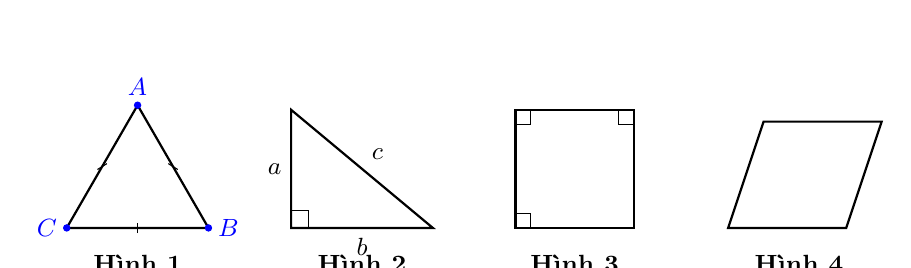
\begin{tikzpicture}[scale=0.75, font=\small]
  \begin{scope}[shift={(0,0)}]
    \coordinate (C) at (0,0); \coordinate (B) at (2.4,0); \coordinate (A) at (1.2, 2.078);
    \draw[thick] (A) -- (B) -- (C) -- cycle;
    \filldraw[blue] (A) circle (1.5pt) node[above] {$A$};
    \filldraw[blue] (B) circle (1.5pt) node[right] {$B$};
    \filldraw[blue] (C) circle (1.5pt) node[left] {$C$};
    \draw ($(A)!0.5!(B) + (-0.08,0.05)$) -- ($(A)!0.5!(B) + (0.08,-0.05)$);
    \draw ($(A)!0.5!(C) + (-0.08,-0.05)$) -- ($(A)!0.5!(C) + (0.08,0.05)$);
    \draw ($(B)!0.5!(C) + (0,-0.09)$) -- ($(B)!0.5!(C) + (0,0.09)$);
    \node at (1.2, -0.6) {\textbf{Hình 1}};
  \end{scope}
  \begin{scope}[shift={(3.8,0)}]
    \coordinate (V) at (0,0); \coordinate (X) at (2.4,0); \coordinate (Y) at (0,2);
    \draw[thick] (V) -- (X) -- (Y) -- cycle; \draw (0,0.3) -- (0.3,0.3) -- (0.3,0);
    \node[left] at (0,1) {$a$}; \node[below] at (1.2,0) {$b$}; \node[above right] at (1.2,1) {$c$};
    \node at (1.2, -0.6) {\textbf{Hình 2}};
  \end{scope}
  \begin{scope}[shift={(7.6,0)}]
    \coordinate (D) at (0,0); \coordinate (C3) at (2,0); \coordinate (B3) at (2,2); \coordinate (A3) at (0,2);
    \draw[thick] (A3) -- (B3) -- (C3) -- (D) -- cycle;
    \draw (0,1.75) -- (0.25,1.75) -- (0.25,2); \draw (2,1.75) -- (1.75,1.75) -- (1.75,2); \draw (0,0.25) -- (0.25,0.25) -- (0.25,0);
    \node at (1, -0.6) {\textbf{Hình 3}};
  \end{scope}
  \begin{scope}[shift={(11.2,0)}]
    \coordinate (D4) at (0,0); \coordinate (C4) at (2,0); \coordinate (B4) at (2.6,1.8); \coordinate (A4) at (0.6,1.8);
    \draw[thick] (A4) -- (B4) -- (C4) -- (D4) -- cycle;
    \node at (1.2, -0.6) {\textbf{Hình 4}};
  \end{scope}
\end{tikzpicture}
\end{center}
\choice
{\True Hình 1}
{Hình 2}
{Hình 3}
{Hình 4}
\loigiai{
Hình 1 có ký hiệu 3 cạnh bằng nhau nên là tam giác đều.
}
\end{ex}

\begin{ex}
Kết quả của $7^{56} : 7^{51}$ viết dưới dạng một lũy thừa là:
\choice
{\True $7^5$}
{$7^6$}
{$7^{107}$}
{$7^4$}
\loigiai{
Khi chia hai lũy thừa cùng cơ số: $7^{56} : 7^{51} = 7^{56 - 51} = 7^5$.
}
\end{ex}

\begin{ex}
Trong các hình dưới đây, hình nào là tam giác đều?
\begin{center}
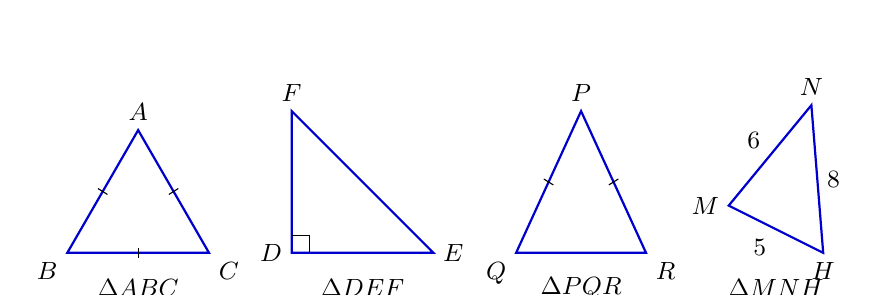
\begin{tikzpicture}[scale=0.75, font=\small]
  \begin{scope}[shift={(0,0)}]
    \coordinate (B) at (0,0); \coordinate (C) at (2.4,0); \coordinate (A) at (1.2, 2.078);
    \draw[thick, blue!80!black] (A) -- (B) -- (C) -- cycle;
    \node[above] at (A) {$A$}; \node[below left] at (B) {$B$}; \node[below right] at (C) {$C$};
    \draw ($(A)!0.5!(B) + (-0.08,0.05)$) -- ($(A)!0.5!(B) + (0.08,-0.05)$);
    \draw ($(A)!0.5!(C) + (-0.08,-0.05)$) -- ($(A)!0.5!(C) + (0.08,0.05)$);
    \draw ($(B)!0.5!(C) + (0,-0.09)$) -- ($(B)!0.5!(C) + (0,0.09)$);
    \node at (1.2, -0.6) {$\Delta ABC$};
  \end{scope}
  \begin{scope}[shift={(3.8,0)}]
    \coordinate (D) at (0,0); \coordinate (E) at (2.4,0); \coordinate (F) at (0,2.4);
    \draw[thick, blue!80!black] (D) -- (E) -- (F) -- cycle; \draw (0,0.3) -- (0.3,0.3) -- (0.3,0);
    \node[left] at (D) {$D$}; \node[right] at (E) {$E$}; \node[above] at (F) {$F$};
    \node at (1.2, -0.6) {$\Delta DEF$};
  \end{scope}
  \begin{scope}[shift={(7.6,0)}]
    \coordinate (Q) at (0,0); \coordinate (R) at (2.2,0); \coordinate (P) at (1.1,2.4);
    \draw[thick, blue!80!black] (P) -- (Q) -- (R) -- cycle;
    \node[above] at (P) {$P$}; \node[below left] at (Q) {$Q$}; \node[below right] at (R) {$R$};
    \draw ($(P)!0.5!(Q) + (-0.08,0.05)$) -- ($(P)!0.5!(Q) + (0.08,-0.05)$);
    \draw ($(P)!0.5!(R) + (-0.08,-0.05)$) -- ($(P)!0.5!(R) + (0.08,0.05)$);
    \node at (1.1, -0.6) {$\Delta PQR$};
  \end{scope}
  \begin{scope}[shift={(11.2,0)}]
    \coordinate (M) at (0,0.8); \coordinate (H) at (1.6,0); \coordinate (N) at (1.4,2.5);
    \draw[thick, blue!80!black] (M) -- (H) -- (N) -- cycle;
    \node[left] at (M) {$M$}; \node[below] at (H) {$H$}; \node[above] at (N) {$N$};
    \node[below left] at (0.8,0.4) {$5$}; \node[above left] at (0.7,1.6) {$6$}; \node[right] at (1.5,1.25) {$8$};
    \node at (0.8, -0.6) {$\Delta MNH$};
  \end{scope}
\end{tikzpicture}
\end{center}
\choice
{\True Tam giác $ABC$}
{Tam giác $DEF$}
{Tam giác $PQR$}
{Tam giác $MNH$}
\loigiai{
Tam giác $ABC$ có ký hiệu ba cạnh bằng nhau nên là tam giác đều.
}
\end{ex}

\begin{ex}
Cho hình bình hành $AKHE$ có $AK = 6\text{ cm}, KH = 5\text{ cm}$. Hãy chọn phát biểu đúng trong các phát biểu sau:
\choice
{$EH = 5\text{ cm}, AE = 6\text{ cm}$}
{\True $EH = 6\text{ cm}, AE = 5\text{ cm}$}
{$AH = 6\text{ cm}, AE = 5\text{ cm}$}
{$KH = 6\text{ cm}, AH = 5\text{ cm}$}
\loigiai{
Trong hình bình hành $AKHE$, các cạnh đối bằng nhau: $EH = AK = 6\text{ cm}$ và $AE = KH = 5\text{ cm}$.
}
\end{ex}

\begin{ex}
Tập hợp $L = \{x \in \mathbb{N}^* \mid x \text{ là số lẻ và } x \le 9\}$ được viết dưới dạng liệt kê các phần tử là:
\choice
{$\{1; 3; 5; 7\}$}
{\True $\{1; 3; 5; 7; 9\}$}
{$\{1; 2; 3; 4; 5; 6; 7; 8\}$}
{$\{1; 2; 3; 4; 5; 6; 7; 8; 9\}$}
\loigiai{
Các số tự nhiên khác 0, là số lẻ và nhỏ hơn hoặc bằng 9 là $1; 3; 5; 7; 9$. Do đó $L = \{1; 3; 5; 7; 9\}$.
}
\end{ex}

\begin{ex}
Chu vi hình thoi $MNPQ$ có cạnh $MN = 5\text{ cm}$ là:
\choice
{\True $20\text{ cm}$}
{$15\text{ cm}$}
{$25\text{ cm}$}
{$10\text{ cm}$}
\loigiai{
Hình thoi có 4 cạnh bằng nhau nên chu vi là: $4 \times 5 = 20\text{ (cm)}$.
}
\end{ex}


\setcounter{ex}{0}
\vspace{2mm}
\noindent\textbf{\large PHẦN II. CÂU TRẮC NGHIỆM ĐÚNG SAI}
\vspace{1mm}
\begin{ex}
Xét tính đúng/sai của các mệnh đề sau:
\choiceTF
{Mọi số có chữ số tận cùng là 3; 6; 9 thì chia hết cho 3}
{Để số $\overline{212*}$ chia hết cho 2 thì $* \in \{4; 6; 8\}$}
{\True Số chia hết cho 9 thì số đó chia hết cho 3}
{\True Các số có chữ số tận cùng là 0 hoặc 5 thì chia hết cho 5}
\loigiai{
\textbf{a)} Sai. Dấu hiệu chia hết cho 3 phụ thuộc vào tổng các chữ số chứ không phụ thuộc vào chữ số tận cùng. Ví dụ 13 tận cùng là 3 nhưng không chia hết cho 3.

\textbf{b)} Sai. Để chia hết cho 2 thì chữ số tận cùng phải là chẵn, tức là $* \in \{0; 2; 4; 6; 8\}$ (thiếu 0 và 2).

\textbf{c)} Đúng. Vì 9 chia hết cho 3 nên mọi số chia hết cho 9 đều chia hết cho 3.

\textbf{d)} Đúng. Đây là dấu hiệu nhận biết chia hết cho 5.
}
\end{ex}

\begin{ex}
Cho các số $a = 12, b = 18$ và $c = 30$. Xét tính đúng/sai của các mệnh đề sau:
\choiceTF
{\True Số $a$ là bội của 4}
{\True Số 6 là ước chung của cả ba số $a, b, c$}
{Ước chung lớn nhất của $a$ và $b$ là 12}
{\True Bội chung nhỏ nhất của $a$ và $b$ là 36}
\loigiai{
\textbf{a)} Đúng. $12 = 4 \cdot 3$ nên 12 là bội của 4.

\textbf{b)} Đúng. Cả 12, 18, 30 đều chia hết cho 6.

\textbf{c)} Sai. $ƯCLN(12, 18) = 6$ chứ không phải 12.

\textbf{d)} Đúng. $BCNN(12, 18) = 36$.
}
\end{ex}


\setcounter{ex}{0}
\vspace{2mm}
\noindent\textbf{\large PHẦN III. CÂU HỎI TRẢ LỜI NGẮN}
\vspace{1mm}
\begin{ex}
Một hình lục giác đều có độ dài một cạnh bằng $5\text{ cm}$. Tính chu vi của hình lục giác đều đó (theo đơn vị $\text{cm}$). \shortans{30}
\loigiai{
Chu vi hình lục giác đều là: $5 \times 6 = 30\text{ (cm)}$.
}
\end{ex}

\begin{ex}
Một khu vườn hình chữ nhật có chiều dài $15\text{ m}$ và chiều rộng $10\text{ m}$. Người ta làm hàng rào xung quanh khu vườn và để lại một cửa ra vào rộng $2\text{ m}$. Tính độ dài của hàng rào đó (theo đơn vị $\text{m}$). \shortans{48}
\loigiai{
Chu vi khu vườn là: $(15 + 10) \cdot 2 = 50\text{ (m)}$.\\Độ dài hàng rào là: $50 - 2 = 48\text{ (m)}$.
}
\end{ex}


\setcounter{ex}{0}
\vspace{2mm}
\noindent\textbf{\large PHẦN IV. TỰ LUẬN (BÀI TẬP VÀ BAREM ĐIỂM)}
\vspace{1mm}
\begin{ex} (1,0 điểm)
Tìm số tự nhiên $x$, biết:
\begin{enumerate}[label=\textbf{\alph*)}, leftmargin=0.8cm, itemsep=2pt]
\item (0,5 điểm) $x + 37 = 50$
\item (0,5 điểm) $(x + 2) : 5 = 6$
\end{enumerate}
\loigiai{
\textbf{a)} \textbf{[0,5 điểm]}\\ $x = 50 - 37 \Rightarrow x = 13$.

\textbf{b)} \textbf{[0,5 điểm]}\\ $x + 2 = 6 \cdot 5 = 30 \Rightarrow x = 30 - 2 = 28$.


}
\end{ex}
\vspace{2mm}

\begin{ex} (1,0 điểm)
Tập hợp và bài toán thực tế tiết kiệm:
\begin{enumerate}[label=\textbf{\alph*)}, leftmargin=0.8cm, itemsep=2pt]
\item (0,5 điểm) Viết tập hợp $A$ các số tự nhiên nhỏ hơn 8. Liệt kê các số nguyên tố trong tập hợp $A$?
\item (0,5 điểm) Mỗi tháng An tiết kiệm $35\,000$ đồng để mua một đôi giày thể thao. Sau 1 năm, An đã mua được đôi giày và còn lại $23\,000$ đồng. Hỏi đôi giày An mua giá bao nhiêu đồng?
\end{enumerate}
\loigiai{
\textbf{a)} \textbf{[0,5 điểm]}\\ $A = \{0; 1; 2; 3; 4; 5; 6; 7\}$.\\Các số nguyên tố trong tập hợp $A$ là: $2; 3; 5; 7$.

\textbf{b)} \textbf{[0,5 điểm]}\\ Số tiền An tiết kiệm trong 1 năm (12 tháng) là: $35\,000 \cdot 12 = 420\,000\text{ (đồng)}$.\\Giá tiền đôi giày là: $420\,000 - 23\,000 = 397\,000\text{ (đồng)}$.


}
\end{ex}
\vspace{2mm}

\begin{ex} (0,5 điểm)
Một khu vườn hình chữ nhật có chiều dài $20\text{ m}$, chiều rộng ít hơn chiều dài $5\text{ m}$. Người ta dự định rào xung quanh khu đất bằng 4 đường dây kẽm gai để trồng rau.
\begin{enumerate}[label=\textbf{\alph*)}, leftmargin=0.8cm, itemsep=2pt]
\item (0,25 điểm) Hỏi cần tất cả bao nhiêu mét dây kẽm gai để rào khu đất trên?
\item (0,25 điểm) Người nông dân thu hoạch được bao nhiêu kg rau trên khu vườn này, biết rằng cứ $1\text{ m}^2$ thu hoạch được $2\text{ kg}$ rau, diện tích lối đi và hệ thống thoát nước là $50\text{ m}^2$?
\end{enumerate}
\loigiai{
\textbf{a)} \textbf{[0,25 điểm]}\\ Chiều rộng khu vườn là: $20 - 5 = 15\text{ (m)}$.\\Chu vi khu vườn là: $(20 + 15) \cdot 2 = 70\text{ (m)}$.\\Số mét dây kẽm gai cần dùng để rào 4 đường là: $70 \cdot 4 = 280\text{ (m)}$.

\textbf{b)} \textbf{[0,25 điểm]}\\ Diện tích khu vườn là: $20 \cdot 15 = 300\text{ (m}^2\text{)}$.\\Diện tích đất thực tế trồng rau là: $300 - 50 = 250\text{ (m}^2\text{)}$.\\Số kg rau thu hoạch được là: $250 \cdot 2 = 500\text{ (kg)}$.


}
\end{ex}
\vspace{2mm}

\begin{ex} (0,5 điểm)
Không thực hiện tính tổng, chứng minh rằng $A = 1 + 4 + 4^2 + 4^3 + \dots + 4^{2021}$ chia hết cho 21.
\loigiai{
Tổng $A$ có $2022$ số hạng. Ta nhóm 3 số hạng liên tiếp vào một nhóm:
\begin{align*}
A &= (1 + 4 + 4^2) + 4^3(1 + 4 + 4^2) + \dots + 4^{2019}(1 + 4 + 4^2)\\
&= 21 + 4^3 \cdot 21 + \dots + 4^{2019} \cdot 21\\
&= 21 \cdot (1 + 4^3 + \dots + 4^{2019}) \ \vdots \ 21 \quad \text{(đpcm)}.
\end{align*}
}
\end{ex}
\vspace{2mm}


\begin{center}
\rule{4cm}{0.4pt}\\
\textit{--- HẾT ---}
\end{center}
\end{document}
